\label{resultats}

\section{Exploration du corpus Charcot : \textsc{OBVIE} et \textsc{TextPair}}
Une première exploration du corpus Charcot à travers l'application OBVIE nous a permis d'identifier les substantifs les plus importants de chaque corpus en utilisant les fréquences brutes ou des méthodes plus fines comme \textsc{TF-IDF}, \textsc{BM25} (détaillées dans la partie \ref{methodo_stat}), \textsc{$\chi$2} ou le \textsc{Test Gamma}. Cependant, l'application ne permet pas de quantifier la pertinence des expressions polylexicales, soit les n-grammes de mots, très fréquentes dans les deux corpus et dont la décomposition entraînerait une perte d'information (p. ex. le terme polysémique \og{}bulbe\fg{} qui a une valeur spécifique dans l'expression figée \textit{bulbe rachidien}). En observant la figure \ref{fig:bulbe}, nous constatons que l'abscisse donne l'information sur les dates de publication des ouvrages compris dans les corpus, alors que l'ordonnée indique le nombre d'occurrences par million de mots, soit \textit{parties par million} (\textit{ppm})\footnote{\textit{Cf.} le guide d'utilisation d'\textsc{OBVIE} détaillé \url{https://obtic.huma-num.fr/obvie//static/aide.html}.}. 
\begin{figure}[!h]
    \centering
    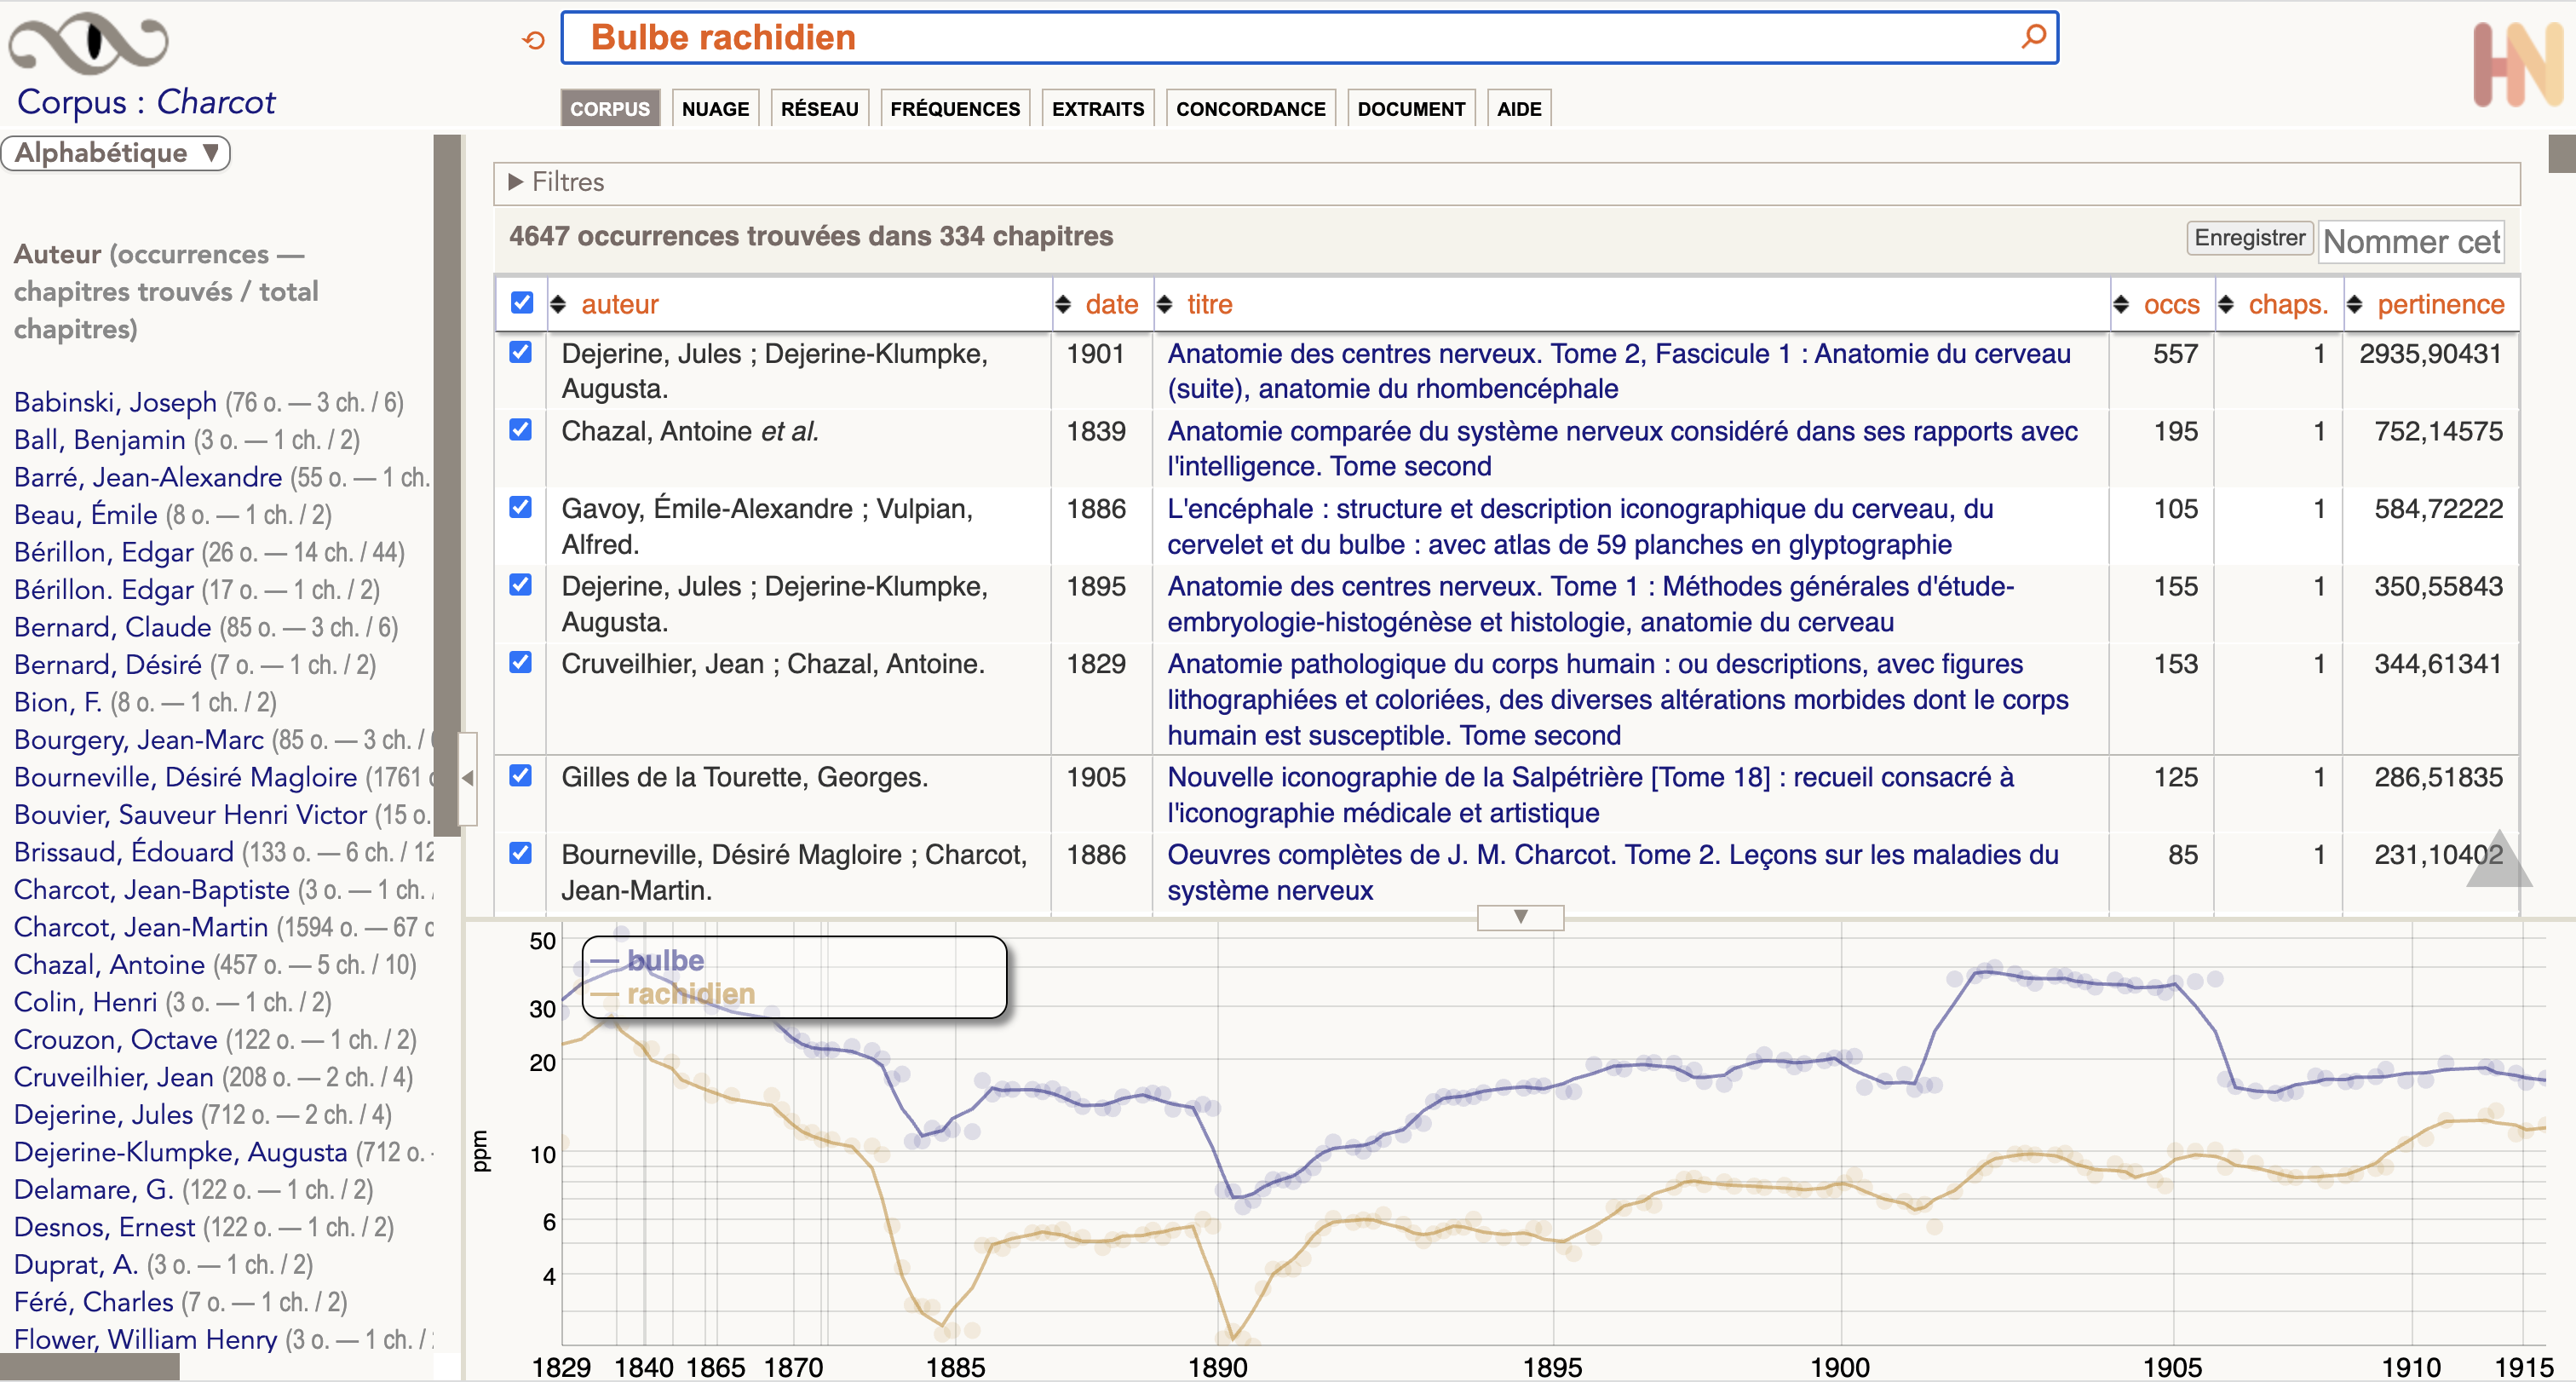
\includegraphics[width=1\textwidth]{img/bulbe_rachidien_mini.png}
    \caption{Distribution des fréquences des tokens avec la frise chronologique pour ceux constituant l'expression \textit{bulbe rachidien} (issus du corpus \og{}Charcot\fg{} et du corpus \og{}Autres\fg{}) dans le logiciel OBVIE.
    % Pour raison de visibilité, l'image originale a été agrandie, ce qui a entraîné le rapprochement des années sur l'axe de l'abscisse.
    }
    \label{fig:bulbe}
\end{figure}

Concernant l'alignement des séquences similaires aux deux corpus, \textsc{TextPair} nous a permis, par une lecture attentive, de faire des comparaisons entre les textes et de rechercher des termes au sein des passages similaires, malgré le nombre de résultats assez conséquent (\textit{cf}. la figure \ref{fig:textpair}).

\begin{figure}[!h]
    \centering
    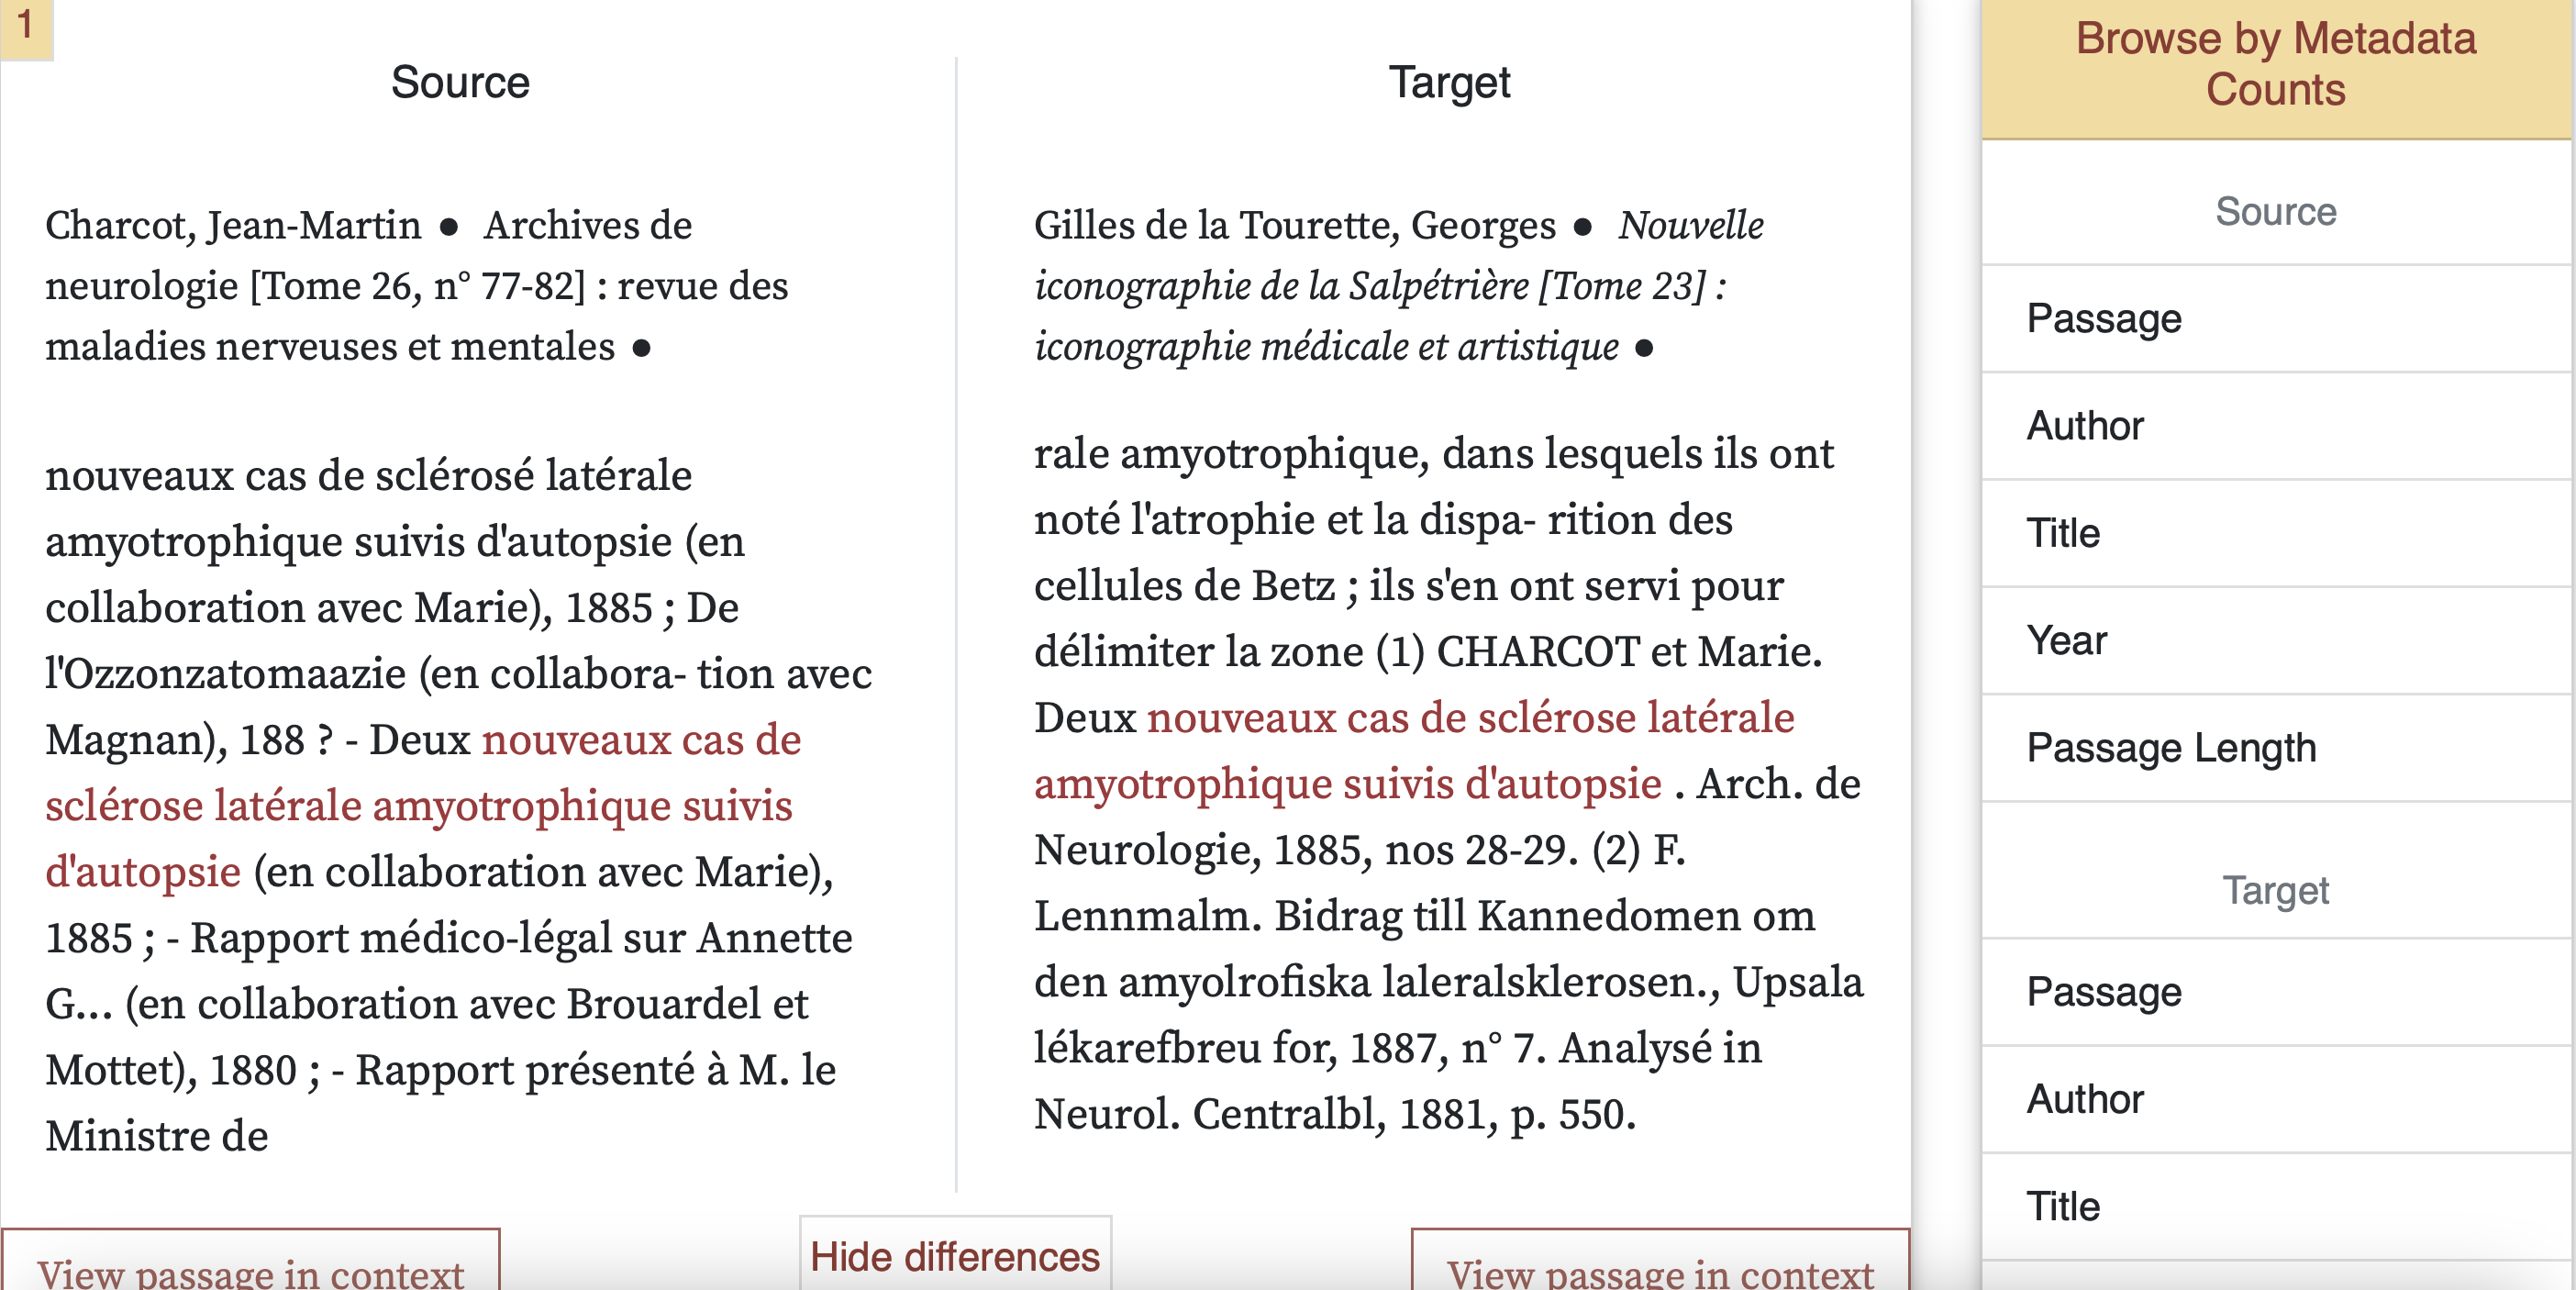
\includegraphics[width=1\textwidth]{img/textpair.png}
    \caption{Alignement et comparaison des textes de Charcot à celui de Georges Gilles de la Tourette (le seul résultat) en lançant la requête \textit{sclérose latérale amyotrophique}.}
    \label{fig:textpair}
\end{figure}
\section{Extraction des phrases-clés : méthodes statistiques}
\label{methodo_stat}
Afin de surmonter les limites rencontrées avec ces deux outils, nous avons proposé une nouvelle méthode pour identifier des concepts dans les deux corpus en nous basant sur le poids de leur apparition, calculé selon trois différentes mesures de pondération\footnote{Le code est disponible en ligne : \url{https://github.com/ljpetkovic/Charcot\_circulations}.} :
\begin{itemize}
\item \textsc{TF-IDF} est une méthode qui permet d'évaluer l'importance d'un terme contenu dans un document relativement à un corpus plus large en récompensant la fréquence des termes, sans tenir compte des variations de longueur du document ;
\item \textsc{BM25} est une fonction de classement qui classe un ensemble de documents en fonction des termes de requête apparaissant dans chaque document, quelle que soit l'interrelation entre les termes de requête au sein d'un document (par exemple, leur proximité relative). Il s'agit d'une tentative d'amélioration de \textsc{TF-IDF}, notamment pour prendre en compte divers facteurs tels que la longueur du document et les problèmes engendrés par la possible saturation des termes \citep{robertson1976relevance} ;
\item \textsc{BERT} \citep{devlin2019} est un modèle pré-entraîné qui utilise l'apprentissage non-supervisé sur de grandes quantités de données textuelles pour apprendre des représentations de mots et de phrases, et comprendre le contexte et la sémantique. Il est basé sur l'architecture des \textit{transformeurs}, qui est un type de réseau de neurones utilisé pour le traitement du langage naturel.
\end{itemize}

La liste des concepts retenus pour l'étude est composée de termes ou expressions popularisés par Charcot \citep{camargo2024}, comme \textit{hystérie}, \textit{sclérose latérale} etc. Pour chaque entrée, nous avons pris en compte les formes du singulier et du pluriel obtenues grâce à des expressions régulières. La liste provient du croisement entre la liste des termes obtenus avec OBVIE et l'index d'une édition des \oe{}uvres complètes de \citet{charcot1892oeuvres}, dont nous avons retiré les termes génériques (\textit{os}, \textit{cerveau}, etc.).

Comme nous pouvons l'observer sur la figure \ref{fig:bm25}, la mesure \textsc{BM25} révèle une intensification du lexique de Charcot dans le corpus \og{}Autres\fg{}. Autrement dit, tous les termes évalués sont identifiés comme plus signifiants dans le discours des \og{}Autres\fg{} que dans celui de Charcot, les scores étant plus élevés pour 14 termes (sur 14 évalués) utilisés par le réseau de Charcot. D'ailleurs, d'après le tableau \ref{tab:calculs_stat} (en annexe), c'est la seule mesure dont les valeurs témoignent clairement d'un lexique partagé entre Charcot et ses successeurs et collaborateurs, \textit{a contrario} des deux autres mesures, où le rapport en question est inversé (la grande majorité des termes étant plus pertinente dans le discours de Charcot, et son impact étant donc moins accentué). Concrètement, les termes les plus pertinents semblent être \textit{sclérose en plaque disséminées} (score 0,83), \textit{paralysie rhumatismale} (0,68), \textit{atrophie progressive} (0,53) et \textit{arthrite déformante} (0,50).

\begin{figure}[!h]
    \centering
    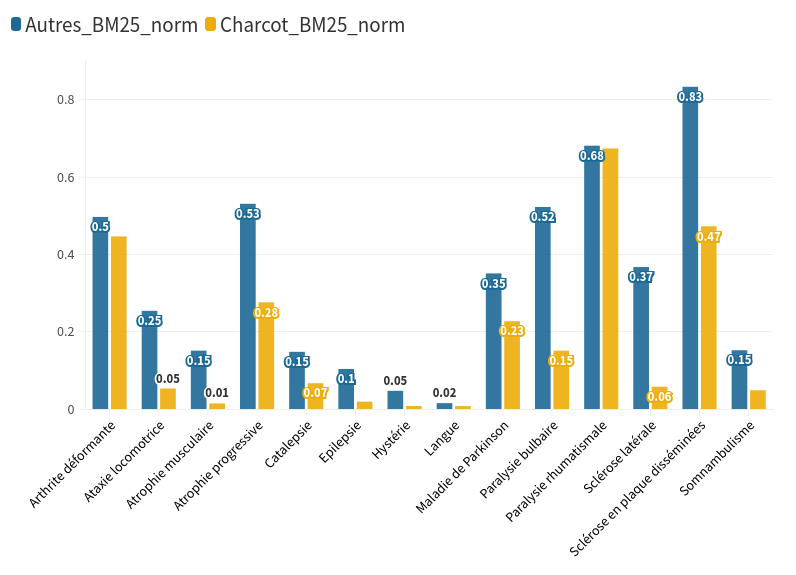
\includegraphics[width=1\textwidth]{img/Charcot_Autres_250523.png}
    \caption{Visualisation de pertinence des concepts dans les deux corpus suivant la métrique \textsc{BM25}. Les valeurs des concepts associées au corpus \og{}Autres\fg{} sont représentées en bleu, alors que celles du corpus \og{}Charcot\fg{} en jaune.}
    \label{fig:bm25}
\end{figure}

D'autre part, nous avons utilisé \textsc{BERT} pour mesurer le poids des termes dans les deux corpus. Bien que ce type de modèle ne fournisse pas directement de poids pour les mots, nous pourrions cependant en extraire des informations utiles pour estimer l'importance ou le poids des mots dans les textes. Différentes approches sont généralement utilisées pour obtenir une représentation de l'importance des mots, en exploitant les informations des plongements lexicaux et des mécanismes d'attention \citep{vaswani2023}. Pour ce travail en cours, nous avons utilisé le modèle \texttt{bert-base-multilingual-cased}. Les premiers résultats obtenus se trouvent dans le tableau \ref{tab:calculs_stat} et restent à améliorer. Cependant, nous avons observé que les termes les plus pertinents pour le discours de Charcot étaient ceux qui désignent les noms des différentes pathologies (\textit{diplopie}, \textit{myélite partielle}, \textit{état de mal épileptique}, \textit{paralysie labio-glosso-laryngée} etc.), contrairement à d'autres notions plus abstraites (\textit{préambule}, \textit{délire}, \textit{miracle}) qui sont prédominantes dans le corpus
\og{}Autres\fg{} (termes non renseignés dans le tableau en question).
\section{Extraction des phrases-clés : méthode à base d'apprentissage profond}


